\documentclass{beamer}

\usepackage[latin1]{inputenc}
\usepackage{listings}
\usepackage{xcolor}

\usetheme{Warsaw}

\title{Effiziente Programme}
\author{F. Gruber, P. H\"onisch, C. Hochreiner, M. Petritsch}
\date{21. 1. 2011}

\begin{document}

\frame{\titlepage}

\begin{frame}\frametitle{Test Set-Up}
\begin{itemize}
  \item Prozessor: i7
  \item Testprogramm: papiex
  \item Testscript: testet gleichzeitig auf o0 und o3
  \item Versionskontrolle: git
\end{itemize}
\end{frame}

\begin{frame}\frametitle{Replaced computation with temp}
\begin{center}
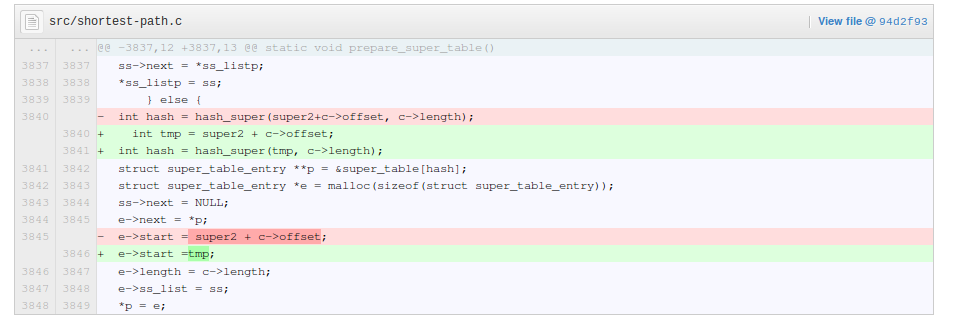
\includegraphics[scale=0.4]{shots/rcwt.png}
\end{center}
\end{frame}

\begin{frame}\frametitle{Replaced computation with temp}
\begin{center}
Result
\end{center}
\end{frame}

\begin{frame}\frametitle{Inline method}
\begin{center}
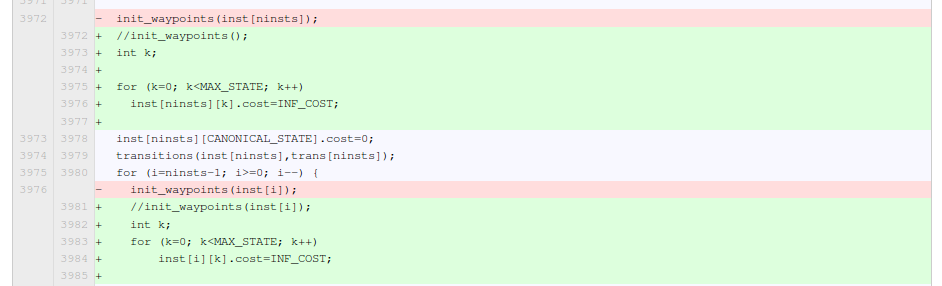
\includegraphics[scale=0.4]{shots/inline.png}
\end{center}
\end{frame}

\begin{frame}\frametitle{Inline method}
\begin{center}
Result
\end{center}
\end{frame}

\begin{frame}\frametitle{Make global constants makros}
\begin{center}
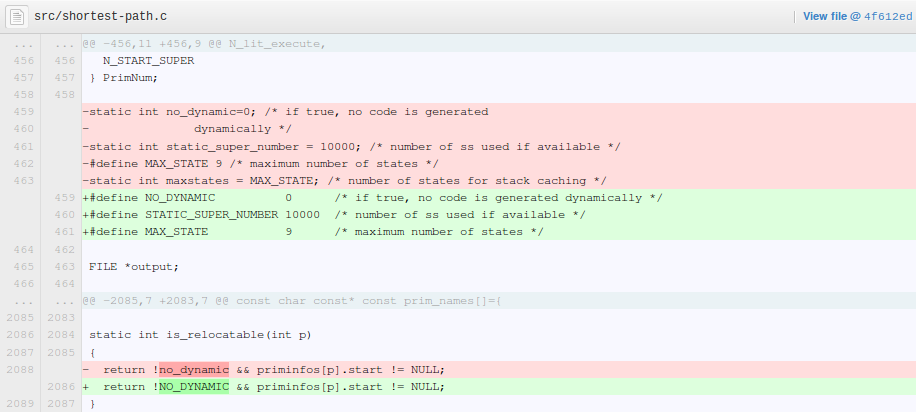
\includegraphics[scale=0.4]{shots/mgcm1.png}
\end{center}
\end{frame}

\begin{frame}\frametitle{Make global constants makros}
\begin{center}
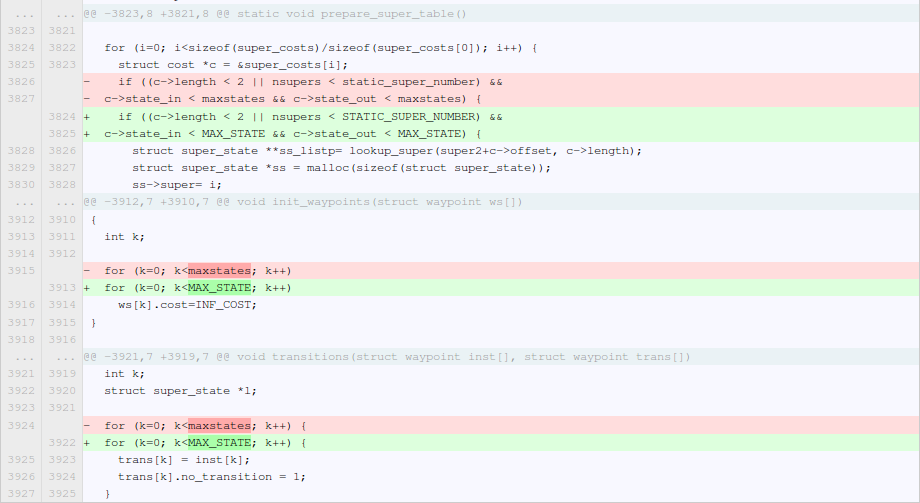
\includegraphics[scale=0.4]{shots/mgcm2.png}
\end{center}
\end{frame}

\begin{frame}\frametitle{Make global constants makros}
\begin{center}
Result
\end{center}
\end{frame}

\begin{frame}\frametitle{Removed function pointer}
\begin{center}
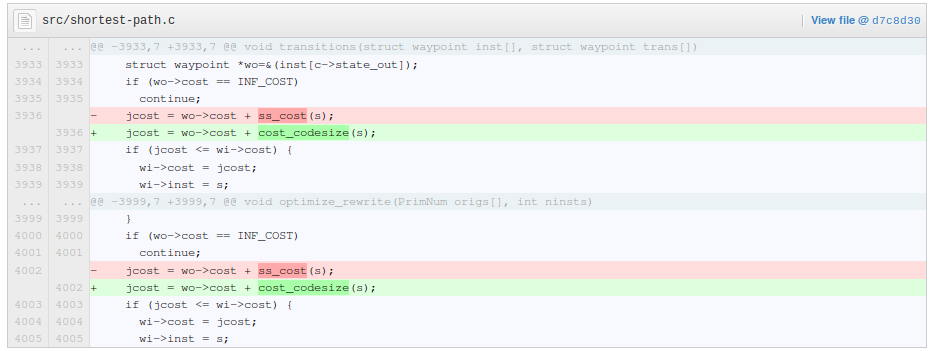
\includegraphics[scale=0.4]{shots/fp.png}
\end{center}
\end{frame}

\begin{frame}\frametitle{Removed function pointer}
\begin{center}
Result
\end{center}
\end{frame}

\begin{frame}\frametitle{Removed is relocateable}
\begin{center}
Result
\end{center}
\end{frame}

\begin{frame}\frametitle{Pointer Arithmetik}
\begin{center}
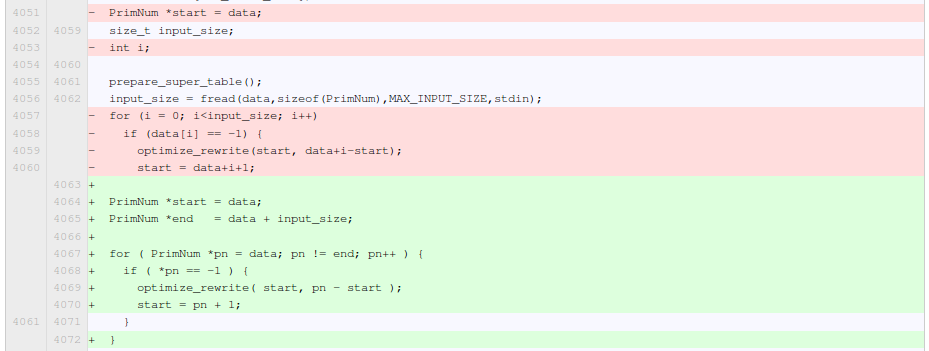
\includegraphics[scale=0.4]{shots/pointer_arith.png}
\end{center}
\end{frame}

\begin{frame}\frametitle{Pointer Arithmetik}
\begin{center}
Result
\end{center}
\end{frame}

\begin{frame}\frametitle{Loop indices}
\begin{center}
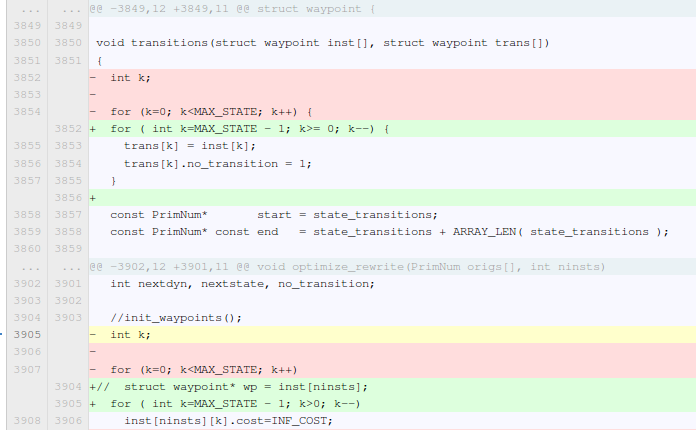
\includegraphics[scale=0.4]{shots/loop_indices.png}
\end{center}
\end{frame}

\begin{frame}\frametitle{Loop indices}
\begin{center}
Result
\end{center}
\end{frame}

\begin{frame}\frametitle{Basic blocks}
\begin{center}
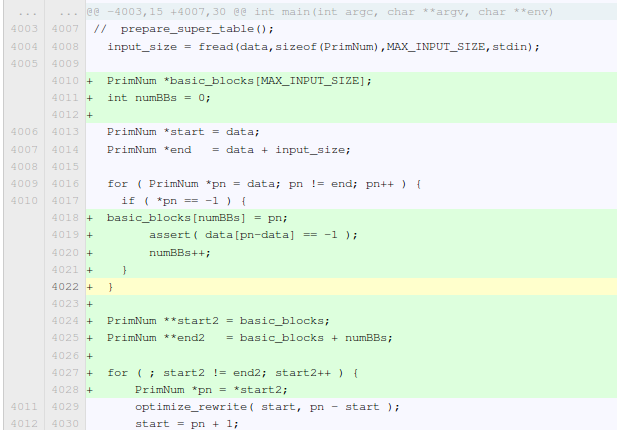
\includegraphics[scale=0.4]{shots/base_block.png}
\end{center}
\end{frame}

\begin{frame}\frametitle{Basic blocks}
\begin{center}
Result
\end{center}
\end{frame}

\begin{frame}\frametitle{Inline cost codesize}
\begin{center}
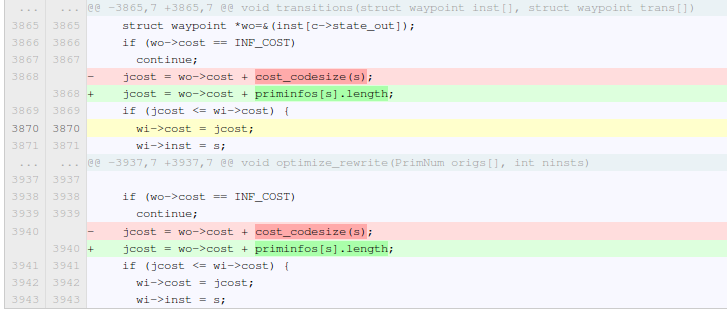
\includegraphics[scale=0.4]{shots/ccs_inline.png}
\end{center}
\end{frame}

\begin{frame}\frametitle{Inline cost codesize}
\begin{center}
Result
\end{center}
\end{frame}

\begin{frame}\frametitle{Inlined generated hashfunction into lookup super.}
\begin{center}
Result
\end{center}
\end{frame}

\begin{frame}\frametitle{Global arrays to constants}
\begin{center}
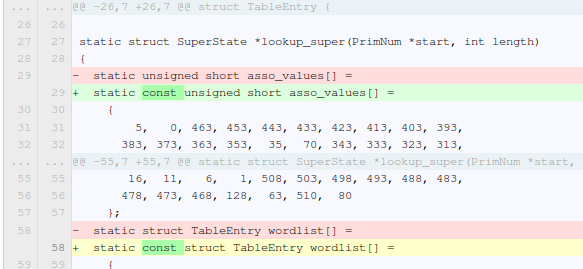
\includegraphics[scale=0.4]{shots/const.png}
\end{center}
\end{frame}

\begin{frame}\frametitle{Global arrays to constants}
\begin{center}
Result
\end{center}
\end{frame}

\begin{frame}\frametitle{Printinst buffer}
\begin{center}
Result
\end{center}
\end{frame}

\begin{frame}\frametitle{Printinst basic block into buffer}
\begin{center}
Result
\end{center}
\end{frame}

\begin{frame}\frametitle{Printinst fputs replaced with write}
\begin{center}
Result
\end{center}
\end{frame}

\begin{frame}\frametitle{Printinst fputs replaced with fwrite}
\begin{center}
Result
\end{center}
\end{frame}

\begin{frame}\frametitle{Whole output into buffer}
\begin{center}
Result
\end{center}
\end{frame}

\begin{frame}\frametitle{Ultimate optimisation}
\begin{center}
Result
\end{center}
\end{frame}

\end{document}